%!TeX root = ../SimplifyJapanese.tex
\begin{frame}[fragile]{Метрики}%
  Метрики BLEU и SARI обученных моделей:
  \begin{table}[H]
    \centering\small
    \label{metrics}
      \begin{tabular}{|l|l|l|}
        \hline
        \textbf{Модель} & \textbf{BLEU} & \textbf{SARI} \\ \hline
        Transformer & 46{,}98 & 64{,}57 \\ \hline
        Pretrained Transformer & \textbf{51{,}12} & \textbf{67{,}89} \\ \hline
        Pretrained Encoder & 48{,}22 & 65{,}67 \\ \hline
      \end{tabular}
      \normalsize
  \end{table}
  Сравнение гистограмм метрик BLEU и SARI ({\color{mathematicaYellow}Transformer} / {\color{mathematicaBlue}Pretrained Transformer}):
  \begin{figure}[H]%
    \centering%
    \label{metrics-comparison}
    % \begin{subfigure}[H]{0.45\textwidth}
    %   \label{bleu-part}
      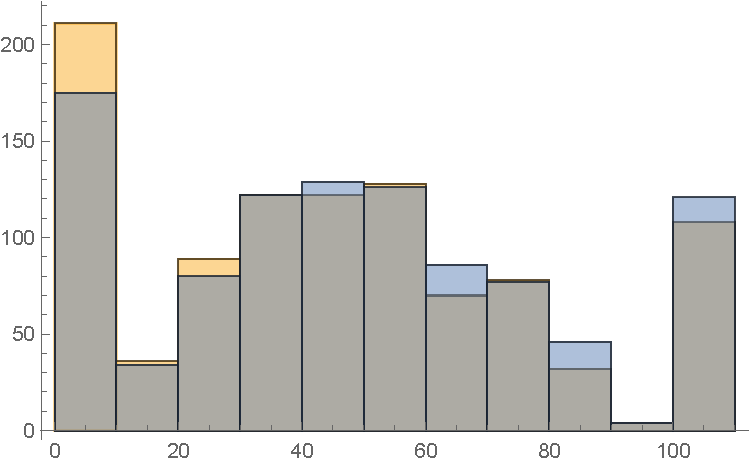
\includegraphics[width=0.3\textwidth]{bleu-comparison.pdf}
    %   \caption{Метрики BLEU}
    % \end{subfigure}
    % \begin{subfigure}[H]{0.45\textwidth}
      % \label{sari-part}
      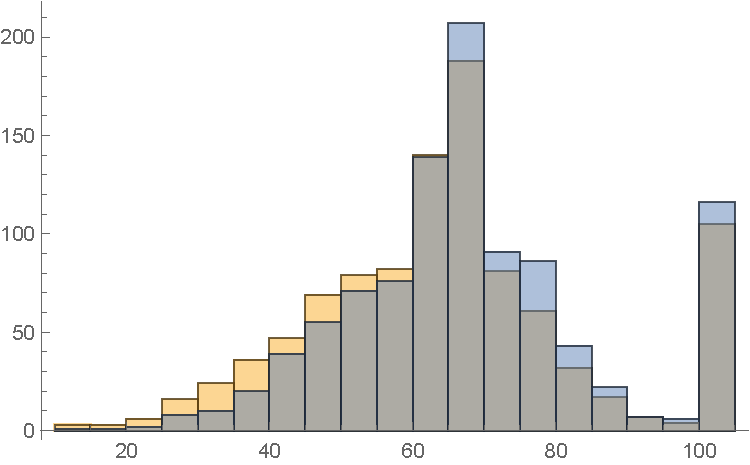
\includegraphics[width=0.3\textwidth]{sari-comparison.pdf}
    %   \caption{Метрики SARI}
    % \end{subfigure}
  \end{figure}%
\end{frame}


\begin{frame}[fragile]{Пример упрощения №1}%
  \sourceSentence{\jpExample{彼は怒りに我を忘れた}{он забылся в гневе}}

  \transformerSample{\jpExample{彼は怒っているのに自分の意見を忘れた}{он хоть и разозлился, но забыл своё мнение}}

  \pretrainedTransformerSample{\jpExample{彼は怒っていることに自分を忘れた}{он забылся, из-за того что разозлился}}

  \notImportant{Интересный момент:} «我» $\to$ «自分», "--- и то, и другое на русском просто «я», но на японском разные оттенки.
\end{frame}


\begin{frame}[fragile]{Пример упрощения №2}%
  \sourceSentence{\jpExample{入場料はただだった}{вход был бесплатным}}

  \transformerSample{\jpExample{入るためのお金はただなかった}{деньги для входа не были бесплатными}}

  \pretrainedTransformerSample{\jpExample{入るためのお金は0円だった}{денег для входа нужно было 0 йен}}

  Здесь происходит замена сложного слова из кандзи (入場料) на простую фразу (入るためのお金).
\end{frame}


\begin{frame}[fragile]{Пример упрощения №3}%
  \sourceSentence{\jpExample{そのスキャンダルはやがてみんなに知れ渡るだろう}{об этом скандале, вероятно, скоро узнают все}}

  \transformerSample{\jpExample{その事件を守る事件はやがてみんなに知られるだろう}{скоро об этом событии, защищающем событие, вероятно, узнают все}}

  \pretrainedTransformerSample{\jpExample{その悪い話はやがてみんなに知られるだろう}{об этой нехорошей истории скоро, вероятно, все узнают}}

  \notImportant{Интересный момент:} в корпусе представлен менее удачный вариант упрощения данного предложения. \\
  その悪い、知られたくないことは、やがてみんなに報告されるだろう \\ 
  "--- Об этом нехорошем деле, о котором никто не хочет знать, скоро всем доложат.
\end{frame}
